\documentclass{article}
\usepackage[utf8]{inputenc}
\usepackage{amsmath}
\usepackage{amsfonts}
\usepackage{amsthm}
\usepackage{graphicx}
\usepackage{setspace}
\usepackage{caption}
\usepackage{subcaption}
\usepackage{listings}
\usepackage{forest}
\usepackage{amsfonts}
\usepackage{array, makecell}
\usepackage{exercise}
\usepackage{kotex}
\usepackage{amssymb}
\usepackage{algorithm}
\usepackage{titlesec}   
\usepackage{algpseudocode}
\usepackage{fancyhdr}
\title{Discrete Mathematics Lecture Note}
\author{TaeYoung Rhee}
\date{October 2022}
\theoremstyle{definition}
\newtheorem{defn}{Definition}[]
\newtheorem{thm}{Theorem}[]
\newtheorem{ex}{Example}[]
\newtheorem{pp}{Proposition}
\newtheorem{nt}{Notation}
\newtheorem*{pf}{Proof}
\newenvironment{pf*}{\pushQED{\qed}\pf}{\popQED\endpf}
\setstretch{1.3}


\begin{document}

\maketitle

\section{Introduction}
Notation.
Define
$ e^x = \sum_{n\ge0} \frac{x^n}{n!}$ e.g.f for $(1,1,1, \cdots)$ \\ 
Define $e^{-x} = \sum_{n\ge0} (-1)^n \frac{x^n}{n!}$ \\ 
Show that $e^x e^{-x} = \left( \sum_{n\ge 0} \frac{x^n}{n!}\right)\left( \sum_{n\ge 0} (-1)^n  \frac{x^n}{n!}\right) = \sum_{n\ge 0} \left( \sum_{i=0}^n (-1)^i { n \choose i} \right) \frac{x^n}{n!}$ = 1. \\ 
Define $\log{1+x} = \sum_{n\ge 1} (-1)^{n-1} \frac{x^n}{n} $ \\ 
\begin{ex}
Generating function for $H_n = 1 + \frac{1}{2} + \cdots + \frac{1}{n}$ with $ H_0 = 0$ 
\begin{align*}
    &\sum_{n\ge 0} H_n x^n = \left( \sum_{n\ge 1} \frac{1}{n}x^n \right) \left( \sum_{n\ge 0 } x^n \right) \\
    & = -\log{(1-x)} \cdot (1-x)^{-1} \\ 
    & = \frac{1}{1-x}\log{\frac{1}{1-x}}
\end{align*}
\end{ex}
\subsection{Infinite Sums and Products in $\mathbb{C}[[x]]$}
\begin{ex}
$p(n) =$ $\#$ of partitions of $n$
\begin{align*}
    \sum_{n\ge 0 } p(n) x^n &= \prod_{i\ge 1} \frac{1}{1-x^i} \\ &= \frac{1}{1-x} \cdot \frac{1}{1-x^2} \cdots 
    \\ &= (1+x+x^2 +\cdots)(1+ x^2 + x^4 + \cdots) \cdots 
\end{align*}
Note that the coefficient of $x^n$ in 첫번째줄 requires finite number of factors. \\ 
\begin{align*}
    &\text{coefficient of } x^n \\ 
    &= \# \text{of solutions} (a_1, a_2, \cdots, a_n) 
    \text{ to } n_1 + 2n_2 + \cdots + = n \\ 
    &= p(n)
\end{align*}
\end{ex}
\begin{defn}
Let $A_0, A_1, \cdots \in \mathbb{C}[[x]]$ \\ 
$A \in \mathbb{C}[[x]]$, $\deg{(A)} = $ first power with nonzero coefficient. 
\end{defn}
The sum $\sum_{i\ge 0} A_i$ exists iff $\deg A_i \rightarrow \infty$.
\begin{align*}
    A_1 &= (a_{10}, a_{11}, a_{12}, a_{13}, \cdots) \\ 
    A_2 &= (0, a_{21}, a_{22}, a_{23}, \cdots) \\ 
    A_3 &= (9, 0, a_{32}, a_{33}, \cdots)
\end{align*}
We can make each row sum is finite.
\begin{ex}
    $e^{1+x}$ is not well-defined. 
    \begin{align*}
        e^{1+x} &= 1+ \left(1+x\right) + \frac{(1+x)^2}{2!} + \frac{(1+x)^3}{3!} + \cdots  
    \end{align*}
    \begin{align*}
        e^{e^x - 1} &= \sum_{n \ge 0} B(n) \frac{x^n}{n!} \\ 
        &= 1 + \left(\sum_{n\ge 1} \frac{x^n}{n!}\right) + \frac{\left(
            \sum_{n\ge 1} \frac{x^n}{n!}
        \right)^2}{2!} + \cdots
    \end{align*}
\end{ex} 
Assume the constant term of each $A_i =1$. 
$ \prod_{i\ge 1} A_i \text{ exists iff } \deg(A_i -1) \rightarrow \infty $
\begin{ex}
    $(1+x)(1+x^2)(1+x^3) \cdots $ is well defined.
    $= \sum_{n \ge 0} p_d(n) x^n$
\end{ex}

Propositions \\ 
(1) $\prod_{i\ge 0} A_i$ and $\prod_{i\ge 0 } B_i$ are well-defined $\Rightarrow \prod_{i\ge 0} A_i B_i = \left(\prod_{i\ge 0} A_i\right)\left(\prod_{i\ge 0} B_i\right)$
\begin{pf*}
    $\deg(AB - 1) \ge \min \{ \deg(A-1), \deg(B-1)\}$
    The factors that contribute to $x^n$ are the same on both sides
\end{pf*} 
(2) $\left( \prod_{i\ge 0} A_i  \right)^{-1} = \prod_{i\ge 0} A_i^{-1}$
\begin{pf*}
     dhotldqkfs
    \begin{align*}
        \deg(A_i - 1) = \deg(A_i^{-1} - 1)
    \end{align*}
    example \\ 
    \begin{align*}
        A = \prod_{i\ge 0} (i - x^{i}) \Rightarrow A^{-1} = \prod_{i\ge 0} \frac{1}{1-x^i}
    \end{align*}
\end{pf*}
(3) $ \frac{\prod_{i\ge 0 } A_i}{\prod_{i \ge 0} B_i} = \prod_{i\ge 0} \frac{A_i}{B_i}$
\begin{ex}
    $\frac{\prod_{i\ge 1}(1-x^{2i})}{\prod_{i\ge 1} (1-z^i)} = \prod_{i \ge 1} = \prod_{i\ge 1} (1+ z^i) = \sum_{n\ge 0} p_d(n) x^n
    = \prod_{i\ge 1} \frac{1}{1-z^{2i-1}} = \sum_{n\ge 0} p_0(n)x^n$ \\ 
    $p_0(n)$ is number of partitions of $n$ where parts are odd.
\end{ex}
\subsection{Compositions in $\mathbb{C}[[x]]$}
$A(x), B(x) \in \mathbb{C}[[x]]$ \\ 
$A(B(x))$ is well-defined if either (1) $A(x)$ is a polynomial or 
(2) the constant term in $B(x) = 0$
\begin{ex}
    \begin{align*}
        A(x) &= e^x \\ 
        B(x) &= e^x - 1
    \end{align*}
    $A(B(x)) = e^{e^{x} - 1}$. \\ 
    When $C(x) = x+1$, $A(C(x)) = e^{x+1}$ is not well defined.
\end{ex}
\subsection{General Powers}
Propositions. Given any $\lambda \in \mathbb{C}$, define 
${\lambda \choose n} = \frac{\lambda(\lambda-1)\cdots(\lambda-n+1)}{n!}$ with ${\lambda \choose 0} = 1$ \\ 
Define $(1+x)^{\lambda} = \sum_{n\ge 0} {\lambda \choose x^n} \in \mathbb{C}[[x]]$ \\ 
If $\lambda$ is a positive integer, this is just the binomial theorem. \\ 
If $A(x) \in \mathbb{C}[[x]]$ with $A(0) = 0$,
then $(1+ A(x))^\lambda = \sum_{n\ge 0} {\lambda \choose n} A(x)$.
\begin{ex}
    \begin{align*}
        (1-x)^{-k} \overset{?}{=} \frac{1}{(1-x)^k}
    \end{align*}
    Note that 
    \begin{align*}
        {-k \choose n} &= \frac{-k (-k -1)(-k -2 ) \cdots (-k-n+1)}{n!}\\ 
        &= \frac{(-1)^n (n+k-1)_n }{n!} \\ 
        &= (-1)^n {n + k - 1 \choose n} = (-1)^n { n+ k - 1\choose k - 1}
    \end{align*} 
    \begin{align*}
        (1-x)^{-k} &= \sum_{n\ge 0} {-k \choose n} (-1)^n x^n \\ 
        &= \sum_{n \ge 0} {n+k -1 \choose k -1} x^n = \frac{1}{(1-x)^k}
    \end{align*}
\end{ex}
Proposition. $(1+x)^\lambda (1+x)^\mu = (1+x)^{\lambda + \mu}$
\begin{ex}
    \begin{align*}
        (1+x)^{\frac{1}{2}} ( 1+ x)^{\frac{1}{2}} = 1 + x
    \end{align*}
\end{ex}
\begin{pf*}
    Need to show 
    \begin{align*}
        \sum_{i=0}^n {\lambda \choose i} {\mu \choose n-i} = 
        {\lambda + \mu \choose \mu} \text{ for all } n \ge 0 
    \end{align*}
    We can prove it in algebra. 
    Otherwise, we can show it by proving coefficient of $x^n$ for LHS $=$ 
    coefficient of $x^n$ for RHS.\\ 
    Check that 
    \begin{align*}
        {x+y \choose n} = \sum_{i=0}^n { x \choose i}{y \choose n - i}
        \text{ for all positive integers } x, y
    \end{align*}
    Let LHS = $f(x, y)$ and RHS = $g(x,y)$. \\ 
    $f(x, y) = g(x, y)$ for infinitely many $x, y$ \\ 
    $f=g$ as polynomials.
\end{pf*} 

\subsection{Catalan Numbers}
\begin{align*}
    &c_0 = 0, c_1 = 1, c_2 = 1, c_3 = 2, c_4 = 5 \\ 
    &c_5 = c_1 c_4 + c_2 c_3 + c_3 c_3 + c_4c_1 \\ 
\end{align*}
\begin{align*}
    c_n = \sum_{i=1}^{n-1} c_i c_{n-i}
\end{align*}
Let $C(x) = \sum_{n\ge 0} c_n x^n$. 
\begin{align*}
    &C(x) = C(x)^2 + x \\ 
    & \Rightarrow C(x)^2 - C(x) = -x \\ 
    & \Rightarrow C(x)^2 - C(x) + \frac{1}{4} = \frac{1}{4} - x\\
    & \Rightarrow \left(C(x) - \frac{1}{2}\right)^2 = \frac{1}{4} - x\\
    & \Rightarrow C(x) - \frac{1}{2} = \pm \frac{1}{2} (1-4x)^{\frac{1}{2}}
\end{align*}
Since $C(x) = c_0 = 0$, we get 
\begin{align*}
    &C(x) - \frac{1}{2} = -\frac{1}{2}(1-4x)^{\frac{1}{2}} \\ 
    &\therefore C(x) = \frac{1}{2} -  \frac{1}{2}(1-4x)^{\frac{1}{2}}
\end{align*}
\begin{align*}
    (1-4x)^{\frac{1}{2}} &= 1 + \sum_{n\ge 1} {\frac{1}{2} \choose n} (-1)^n 4^n x^n \\ 
    &= 1- 2\sum_{n\ge 1}\frac{1}{n}{2n-2 \choose n-1 } x^n
\end{align*}
Check that 
\begin{align*}
    {1\frac{1}{2} \choose n} = \frac{(-1)^{n-1}}{2^{2n-1}}\frac{1}{n}{2n -2 \choose n-1}
\end{align*}
Thus
\begin{align*}
    c_n = \frac{1}{n} {2n-2\choose n-1}
\end{align*}
\subsection{Other interpretations of Catalan Number}
$c_n =$ number of ways to parenthesize a product $x_1 x_2 \cdots x_n$  
\begin{ex}
    For $x_1 x_2 x_3 x_4$, there are 5 ways. \\ 
    Key observation is the outermost parenthesis multiples two terms.
    The first is a product involving $x_1, x_2, \cdots , x_r$ $\rightarrow$ $a_r$ 
    ways to do this. The second is a product involving $x_r+1, x_r+2, \cdots, x_n$ $\rightarrow$
    $a_{n-r}$ ways.
\end{ex}
number of binary trees with $n$ leaves and 1 root. A tree is binary if 
every vertex has degree 1 or 3. \\ 
\begin{figure}[!h]
    \centerline{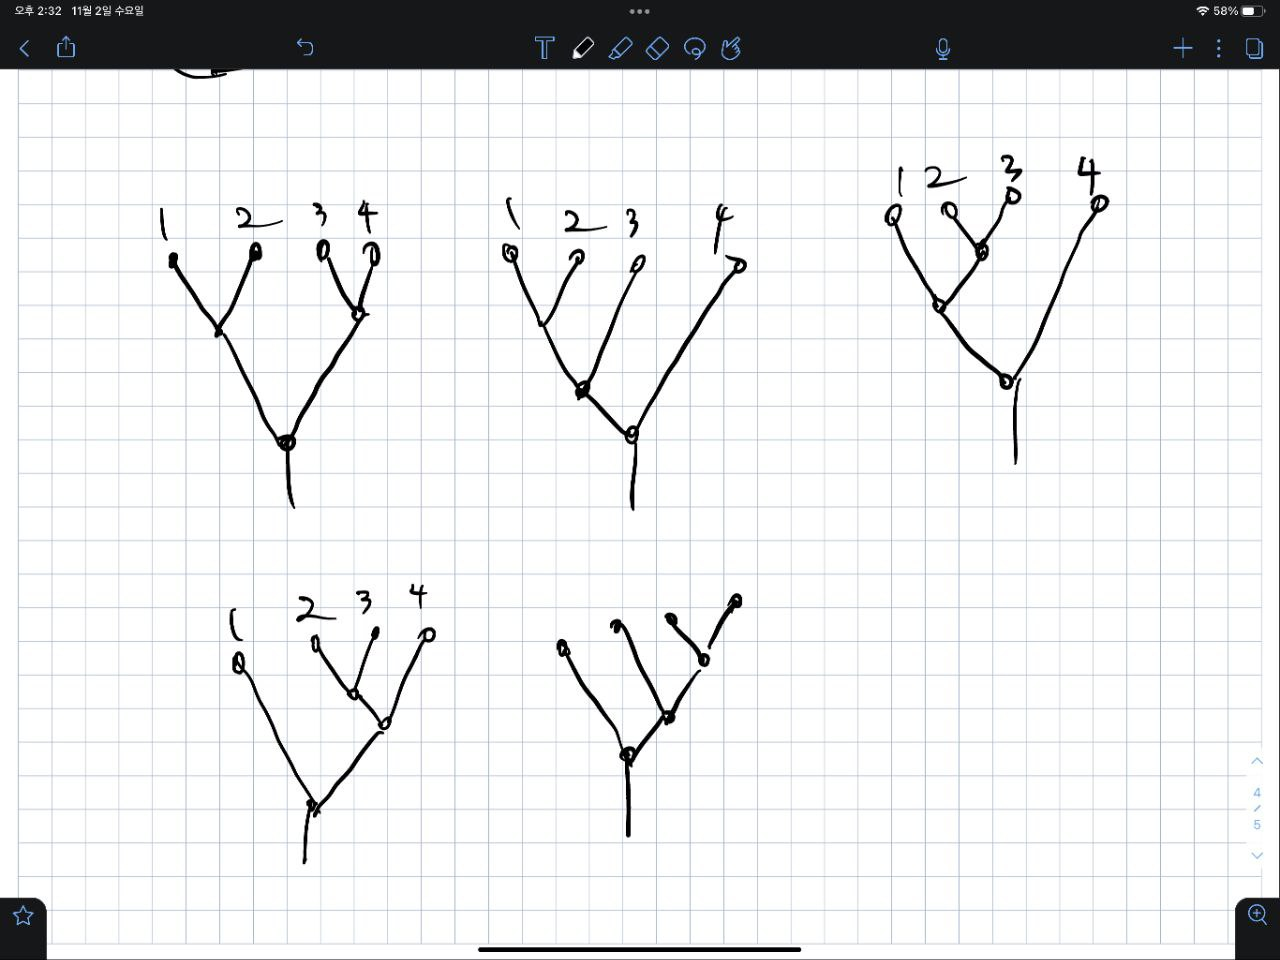
\includegraphics[width=0.5\columnwidth]{tree.jpg}}
    \caption{binary tree}
    \label{tree} 
\end{figure}
A bijections among these sets (triangulations of $n+1$-gon, parenthesized products
of $n$ vatiables, binary trees with $n$ leaves)
\begin{ex}
    Figure \ref{figure_1} is the bijection between the sets.
    \begin{figure}[!h]
        \centerline{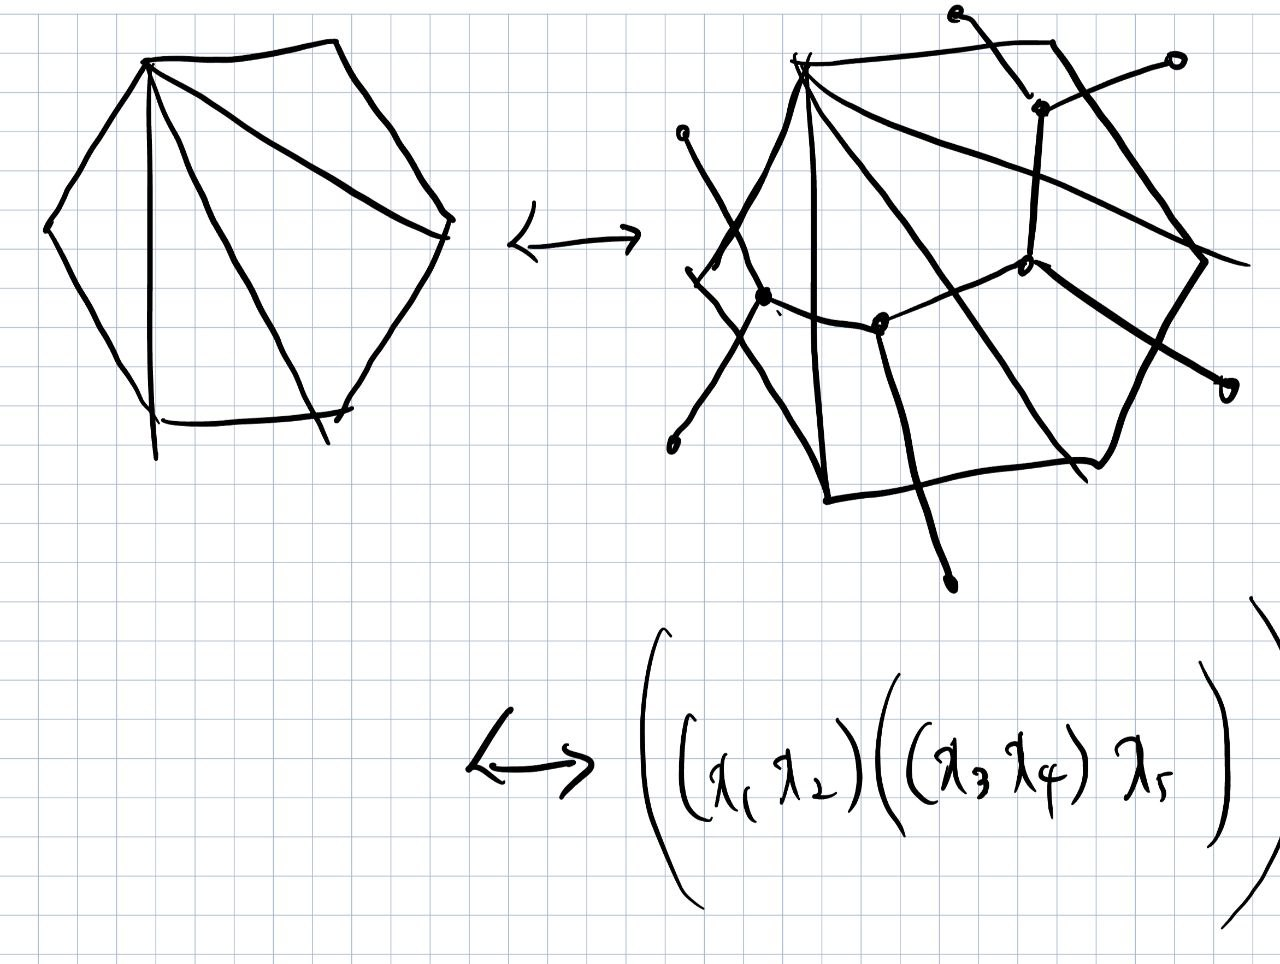
\includegraphics[width=0.5\columnwidth]{bijection_gon.jpg}}
        \caption{bijections}
        \label{figure_1} 
    \end{figure}
\end{ex}
\subsection{Product of exponential generating functions}
\begin{align*}
    A(x) &= \sum_{n\ge 0} a_n \frac{x^n}{n!} \\ 
    B(x) &= \sum_{n\ge 0} b_n \frac{x^n}{n!}
\end{align*}
\begin{align*}
    A(x)B(x) = \sum_{n\ge 0} c_n \frac{x^n}{n!} \text{ where } 
    c_n = \sum_{i=0}^{n} {n \choose i} a_i b_{n-i}
\end{align*}
It means number of ways to partition on $n$-set into 
two ordered blocks and create structure ``$A$'' in the 
first block and structure ``$B$'' in the second block. \\ 
\textbf{Remark} If ``$A$'' = ``$B$'', then $\frac{A(x)^2}{2!} = $ e.g.f
for the number of ways to create two unordered blocks in an $n$-set and create
structure ``$A$'' in each block.\\ 
\textbf{Remark} If both blocks of an $n$-set has to be non-empty then
let $a_0=b_0=0$ 
\begin{ex}
    $c_n = $ number of ways to color $n$ labeled balls with red and blue
    so that an even number of balls are colored red and an odd number of balls
    are colored blue.\\ 
    $c_n = 0$ if $n$ is even. $c_n = 2^{n-1}$ if $n$ is odd.\\
    $R(x) = $ e.g.f for $(1,0,1,0,\cdots) = 1 + \frac{x^2}{2!} + \frac{x^4}{4!} = 
    \frac{e^x + e^{-x}}{2}$\\ 
    $B(x) = $ e.g.f for 
    $(0,1,0,1,\cdots) = x + \frac{x^3}{3!} + \frac{x^5}{5!} + \cdots = 
    \frac{e^x - e^{-x}}{2}$
    \begin{align*}
        \sum_{n\ge 0} c_n \frac{x^n}{n!} &= C(x) = R(x)\cdot B(x) \\ 
        &= \frac{e^{2x} - e^{-2x}}{4} \\ 
        &= \frac{1}{4} \left[\left(1 + 2x + \frac{(2x)^2}{2!} + \cdots \right) - 
        \left(1 - 2x + \frac{(2x)^2}{2!} - \cdots \right)\right]\\ 
        &= \sum_{n\ge 0 \; n \text{ odd}} 2^{n-1} \frac{x^n}{n!}
    \end{align*}
\end{ex}
\begin{ex}
    Dearangement (revisited) 
    \begin{align*}
        P(x) = \sum_{n \ge 0} n! \frac{x^n}{n!} = \sum_{n \ge 0} x^n 
        = \frac{1}{1-x} = \text{ e.g.f for } \{ \vert S_n \vert = n! \} 
    \end{align*}
    \begin{align*}
        I(X) &= \sum_{n\ge 0} 1 \frac{x^n}{n!} = e^x \\ 
        & = \text{ e.g.f for the number of identity permutations on an } n \text{-set} \\ 
        & = \text{ e.g.f for the sequence } (1, 1, 1, \cdots )
    \end{align*}
    \begin{align*}
        D(x) = \sum_{n\ge 0} d_n \frac{x^n}{n!} \text{ where } d_n= 
        \text{ number of dearangements on an } n \text{-set}
    \end{align*}
    $P(x) = I(x)D(x)$ because a permutations on an $n$-set is obtained by 
    \begin{enumerate}
        \item partitioning the $n$-set into two ordered blocks.
        \item create the identity permutations on the first block and
        create a dearangement on the second block.
    \end{enumerate}
    \begin{align*}
        \therefore D(x) = P(x)I(x)^{-1} = \frac{e^{-x}}{1-x}
    \end{align*}
\end{ex}
\end{document} 
